\newpage
\section{Kryptologie}
% TODO: 2 Teile im Pdf?
\section{Grundbegriffe und einfache Verfahren}
	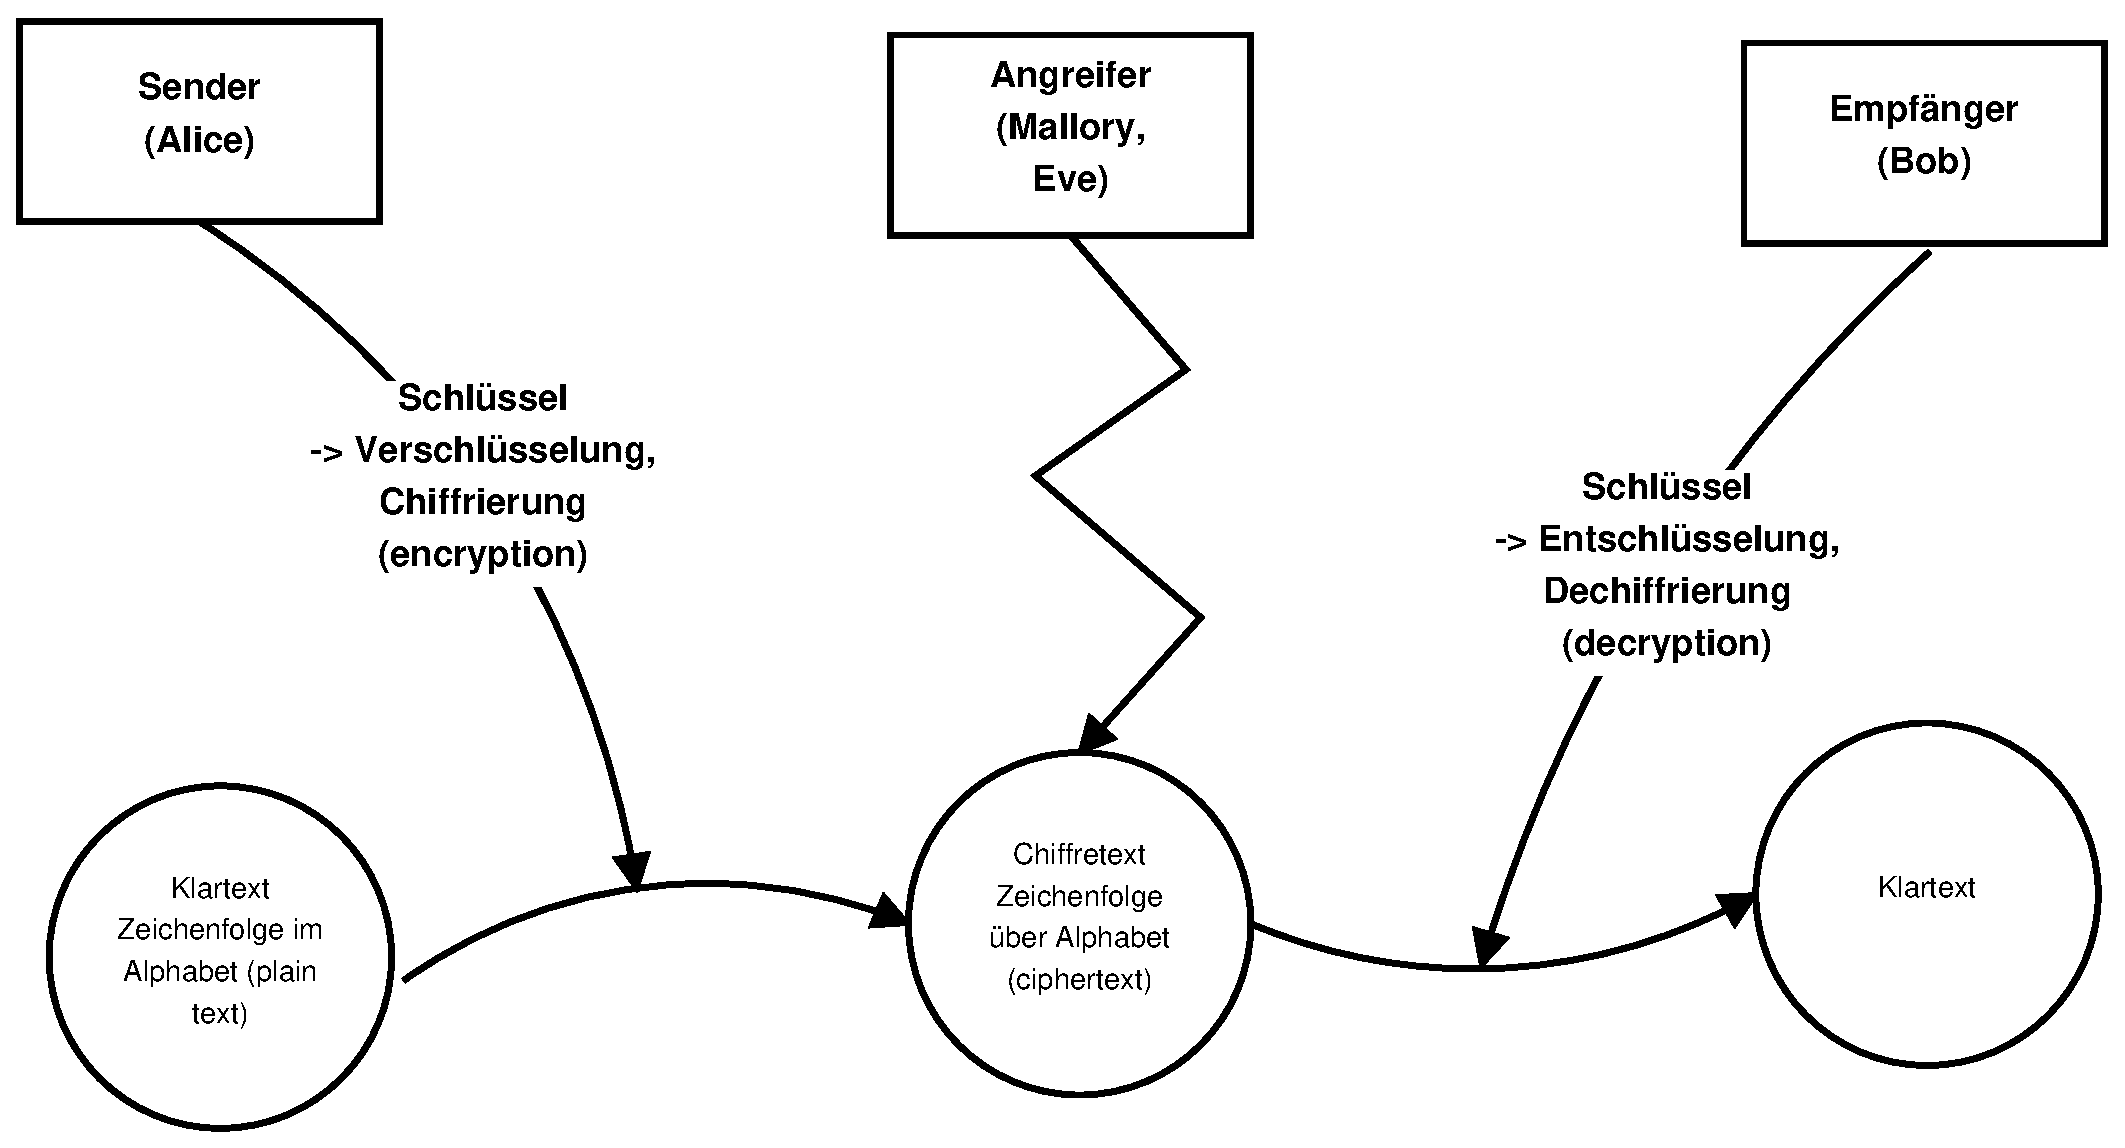
\includegraphics[width=\textwidth]{eps/pic01.eps}

	\textbf{Verschlüsselung erfordert}
	\begin{itemize}
		\item Verschlüsselungsverfahren, Chiffrieralgorithmus (Funktion $E$)
		\item Schlüssel $k_e$ (encryption key)
	\end{itemize}
	$E(\underset{\mbox{\scriptsize Klartext}}{m},\underset{\mbox{\scriptsize Schlüssel}}{k_e})=\underset{\mbox{\scriptsize Chiffretext}}{C}$ \\
	$k_e$ stammt aus der Menge $\mathcal{K}$ von Schlüsseln.\\
	Für ein festes $k_e$ muss $E\lrr{.,k_e}$ injektiv sein, das heißt\\
	$m_1\neq m_2 \Rightarrow E\lrr{m_1,k_e}\neq E\lrr{m_2,k_e}$
	
	\textbf{Entschlüsselung erfordert}
	\begin{itemize}
		\item Entschlüsselungsalgorithmus, Dechiffrierverfahren (Funktion $D$)
		\item Einen von $k_e$ abhängigen Decryption-Key $k_d$
	\end{itemize}
	$D(c,k_d)=m\quad D\lrr{.,k_d}=E\lrr{.,k_e}^{-1}$
	\subsection{Symmetrisches \& Asymmetrisches Verschlüsselungsverfahren}
		Ist $k_d=k_e$, oder falls $k_d$ leicht aus $k_e$ berechenbar ist, so spricht man von einem \textbf{symmetrischen Verschlüsselungsverfahren}.\\
		Lässt sich $k_d$ aus $k_e$ nur mit unverhältnismäßig großem Aufwand berechnen, so kann man $k_e$ öffentlich machen. Das heißt \textbf{Public Key Verfahren} oder auch \textbf{asymmetrisches VerschlÜsselungsverfahren}. (Kein Schlüsselaustausch notwendig!)
	
		In einem symmetrischen Verfahren werden $\binom{n}{2}=\dfrac{n\lrr{n-1}}{2}$ Schlüssel benötigt, wenn $n$ die Anzahl aller Verbindungspaare ist. Bei einem assymmetrischen Verfahren werden lediglich $2n$ Schlüssel benötigt.
	\subsection{Beispiel}
		\subExBegin{a)}
			\item $R=S=\lrc{0,\dots,25}$ \\
				Verfahren - \textbf{Verschiebechiffre}\\
				$\mathcal{K}=\lrc{0,\dots,25}$ \\
				Wähle Schlüssel $i\in\mathcal{K}$\\
				$x\in R$ Verschlüssle $x\rightarrow x+i\mod 26$\\
				$m=x_1\dots x_r\quad x_i\in R$\\
				$E\lrr{m,i}=\underbrace{\lrr{\lrr{x_1+i}\mod 26}}_{y_1}\dots\underbrace{\lrr{\lrr{x_r+i}\mod 26}}_{y_r}=c$\\
				Entschlüssle $y\in R \rightarrow y-i\mod 26$\\
				$D\lrr{c,i}=\lrr{\lrr{y_1-i}\mod 26}\dots\lrr{\lrr{y_r-i}\mod 26}=m$
			\item Verallgemeinerung: \textbf{Zeichenweise Substitutionschiffren}\\
				$R=S=\lrc{0,\dots,25} \quad\mathcal{K}=$ Menge der Permutationen von $R$\\
				Wähle $\pi\in\mathcal{K}$\\
				$m=x_1\dots x_r\quad x_i\in R$\\
				$E\lrr{m,\pi}=\underbrace{\pi\lrr{x_i}}_{y_1}\dots\underbrace{\pi\lrr{x_r}}_{y_r}=c$\\
				$c=y_1\dots y_r$\\
				$D\lrr{c,\pi^{-1}}=\pi^{-1}\lrr{y_1}\dots\pi^{-1}\lrr{y_r}=m$\\
				Jetzt ist $\lrabs{\mathcal{K}}=26!\equiv 4\cdot10^{26}$
			
				Angenommen ein Angreifer kann $10^{12}$ Schlüssel in der Sekunde testen.\\
				Angenommen $50\%$ der Schlüssel getestet werden um den richtigen zu finden.\\
				Dann werden $2\cdot 10^{14}$ Sekunden, also ungefähr $6.000.000$ Jahre benötigt.
		\subExEnd
	\subsection{Bemerkung}
		Das Verfahren aus 1.3b) ist bei Verschlüsselung von natürlichsprachlichen Texten völlig unsicher. Das liegt an der charakteristischen Buchstabenhäufigkeitsverteilung.
	\subsection{Prinzip von Kerkhoffs (1835-1903)}
		Die Sicherheit einer Verschlüsselung darf nicht von der Geheimhaltung des Verfahrens abhängen, sondern nur von der Geheimhaltung des Entschlüsselungsschlüssels $k_d$.
	\subsection{Kryptoanalyse}
		\begin{itemize}
			\item Ciphertext-Only-Angriff
			\item Known-Plaintext-Angriff
			\item Chosen-Plaintext-Angriff
			\item Chosen-Ciphertext-Angriff
	\end{itemize}
\section{One-Time-Pad und perfekte Sicherheit}
	\subsection{Lauftextverschlüsselungen}
		Klartext(über $R=\lrc{0,\dots,25}$) Wähle \textit{Schlüsseltext} der gleichen Länge über $R$\\
		Addiere Schlüsseltext zeichenweise zu Klartext $\mod 26$,
		
		\textbf{Beispiel}
		
		\begin{tabular}{lcccccccccc}
			Klartext&P&E&T&E&R&15&4&19&4&17\\
			Schlüsseltext&H&A&U&C&K&7&0&20&2&10\\\cline{7-11}
			&&&&&&22&4&13&6&1\\
			&&&&&&W&E&N&G&B
		\end{tabular}
		
		Das nennt sich \textbf{kontextabhängiges Verschlüsselungsverfahren}.
	\subsection{One-Time-Pad}
		Klartextalphabet $R=\lrc{0,1}=\mz_2$\\
		Klartext $m$ hat die Länge $n$ über $\mz_2$\\
		Wähle als Schlüsselfolge eine Zufallsfolge $k$ der Länge $n$ und addiere bitweise $\mod 2$ (XOR).\\
		$c=m\oplus k$
		
		\textbf{One-Time-Pad}: Schlüssel nur einmal verwenden.\\
		$c_1=m_1\oplus k$\\
		$c_2=m_2\oplus k$\\
		Angreifer fängt $c_1$ und $c_2$ ab:\\
		$c_1\oplus c_2 = m_1\oplus k\oplus m_2\oplus k=m_1\oplus m_2$\\
		Wenn $m_1,m_2$ sinnvolle Texte sind, so gibt es in $m_1\oplus m_2$ statistische Auffälligkeiten $\Rightarrow$ Angriffsmöglichkeiten.1